\documentclass{report}

\usepackage{global}

\graphicspath{{/home/grybouilli/TIPE/schema/}}

\lhead{Étude cinématique}

\author{Nicolas GRY}

\title{Étude du mouvement du déchet}

\begin{document}
\maketitle
\tableofcontents
\newpage
\chapter{Phase de déplacement dans le champ magnétique}
\section{Mise en situation}
\subsection{Introduction des grandeurs et notations}

On considère un solénoïde caractérisé par:
\begin{itemize}
    \item Sa longueur $L$
    \item Son rayon $a$
    \item L'intensité du courant qui le traverse $i$
    \item Son nombre de spires $n$ 
\end{itemize}
Ce solénoïde engendre un champ magnétique:
 $$\vect{B} = B_r \vect{e_r} + B_z \vect{e_z}$$.
On notera indifféremment $||\vect{B}||$ et $B$.

On considère un déchet spatiale, de masse $m$, que l'on modélise par un moment magnétique solide $\vect{p}$ de moment d'inertie $J_\theta$. 

On notera indifféremment $||\vect{p}||$ et $p$.

On travaillera dans le repère cylindrique $(\vect{e_r},\vect{e_\theta},\vect{e_z})$ et on notera $(r,\theta,z)$ les coordonnées du déchet.

\subsection{Schéma de la situation}

\begin{figure}[h]
    \centering
    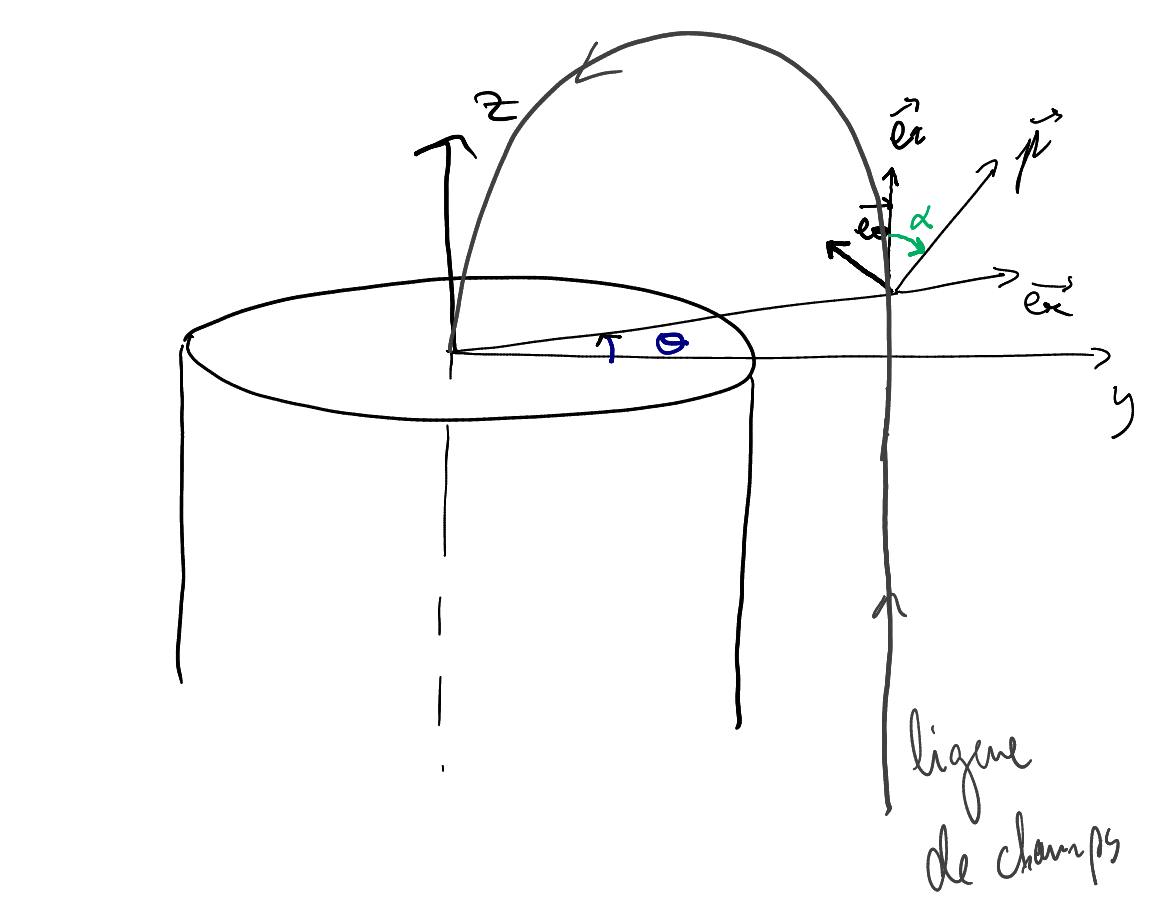
\includegraphics[scale=0.17]{schema_etude_mouvement_1.png}
    \caption{Schéma simplifié de la situation}
\end{figure}  

\section{Étude littérale du mouvement}
\subsection{Étude de l'alignement du déchet}

\ulbf{Système}: {débris assimilé à un moment magnétique solide $\vect{p}$ de moment d'inertie $J_\theta$}

\ulbf{Référentiel}: En lien avec le solénoïde, supposé galiléen (raisonnable au regard de la durée de l'expérience)

\ulbf{Conditions initiales}

À t = 0, on suppose que le déchet est incliné d'un angle $\theta_0$ par rapport à l'axe de révolution du solénoïde. On suppose également la vitesse angulaire du déchet nulle à t = 0, ce qui est raisonnable puisque le déchet est dénué de tout mouvement dû au champ $B$ lorsqu'il n'y est pas soumis, ie à t = 0.

\ulbf{Bilan des forces}

Force magnétique :
$$\vec{F_B} = \vect{\text{grad}}(\vect{B}.\vect{p})$$

\ulbf{Théorème du moment cinétique}

Projeté selon $\vect{e_\theta}$ :
\begin{align*}
J_\theta \derived{\theta}{t} &= \vect{\MM}(\vect{F_B}) . \vect{e_\theta} \\
&= (\vect{p} \wedge \vect{B}).\vect{e_\theta}\\
&= pB_r \cos(\theta) - pB_z\sin(\theta)
\end{align*}

On obtient l'équation différentielle suivante:
\begin{prettybox}[blue]
\ulbf{Équation différentielle du 2$^{nd}$ ordre non-linéaire à second membre non-constant:}
$$\derived{\theta}{t} + \frac{pB_z}{J_\theta}\sin(\theta) = \frac{pB_r}{J_\theta} \cos(\theta)$$
\end{prettybox}
\subsubsection{Étude de la fin de l'alignement}
On se place en premier dans la situation où $\theta$ est considéré petit. On a alors:
$$\derived{\theta}{t} + \frac{pB_z}{J_\theta}\theta = \frac{pB_r}{J_\theta} $$

On pose $$\omega_0 = \sqrt{\frac{pB_z}{J_\theta}}$$

\ulbf{Solution générale de l'équation homogène associée}

$$\theta_h(t) = A \cos(\omega_0 t + \varphi)$$

$\, \text{ avec } A \text{ et } \varphi \text{ des constantes d'intégrations}$.

\newpage
\ulbf{Solution particulière de l'équation}

$$\theta_p(t) = \frac{B_r}{B_z}$$


\ulbf{Solution générale de l'équation}

$$\theta(t) = A \cos(\omega_0 t + \varphi) + \frac{B_r}{B_z}$$

\ulbf{Détermination des constantes d'intégration avec les conditions initiales}

Avec:
$$\theta(0) = \theta_0$$
$$\derive{\theta}{t} (0) = 0$$

On en déduit : 
$$A = \theta_0  - \frac{B_r}{B_z}$$
$$\varphi \equiv 0 \left[\pi\right] $$ 

Et donc finalement :

\begin{prettybox}[blue]
\ulbf{Équation de l'angle formé entre $\vect{p}$ et $\vect{e_z}$}
    $$\theta(t) = \left(\theta_0  - \frac{B_r}{B_z}\right) \cos(\omega_0 t) + \frac{B_r}{B_z}$$
\end{prettybox}
\end{document}